% This is the master examples.tex file -- the most
% up-to-date -- the one on which all others are based.
%
% ICMC2005-examples.tex was integrated on 2005.03.16.
% UHEE616-examples.tex was integrated on 2005.03.16.
% hafg-examples.tex was integrated on 2005.03.16.

%=======================================================================
\subsection{Examples: 1-D Semidirect Product Indexing Sets}
%\protect\footnotemark}
%=======================================================================
%\footnotetext{An and Tolimieri (2003), page 125.}
As seen above, when varying group structures are placed on indexing sets,
and products in the resulting group algebra are computed, 
interesting signal transforms obtain.  In this section,
we elucidate the nature of these operations by
examining some simple, concrete examples in detail.

Recall, in the notation 
%of (\ref{eq:cyclicGroup}) and (\ref{eq:unitGroup}) 
defined above,
%\begin{theorem}
the mapping $\Psi: U(N) \to Aut(C_N(x))$ is a group
isomorphism.
%\end{theorem}
Under this identification, we can form $C_N(x)\sdp K$
for any subgroup $K$ of $U(N)$.  A typical point in 
$C_N(x)\sdp K$ is denoted 
$(x^n, u), \, 0\leq n<N,\, u\in K$ with multiplication given
by  
\[
(x^m, u)(x^n, v) = (x^{m+un},uv), \quad 
0\leq m, n < N,\, u, v \in K
\]
where $m+un$ is taken modulo $N$.
We often use $k_u$ to denote the element $u\in K$ as this
avoids confusion that can arise at various places.

\begin{example}\protect\hspace{-1mm}\footnotemark
\footnotetext{An and Tolimieri (2003), page 125.}
\label{ex:g2}
Let $G_1$ be the abelian group 
\begin{equation}
G_1 = C_{2N}(x) = \{x^n : 0 \leq n < 2N\}. % = \{1, x, x^2, \ldots, x^{2N-1}\}
\end{equation}
Let $G_2$ be the \emph{dihedral group} %$\vs{D}_{2N}(x, k_{N-1})$,
%and suppose the elements of $G_2$ are indexed as follows:
with elements
\begin{eqnarray*}
G_2&=& C_N(x) \sdp \{1, k_{N-1}\}\\
&=& \{x^n k_{N-1}^j : 0 \leq n < N, 0 \leq j < 2\}.
\end{eqnarray*}
We order the elements of $G_2$ as follows:
\[
\{1, x, \ldots, x^{N-1}, k_{N-1}, xk_{N-1}, \ldots, x^{N-1}
k_{N-1}\}
\]
Thus, $G_2$ is divided into two blocks with $N$-samples per block.
\end{example}

\begin{example}\label{ex:g3}
Another group, $G_3$, will be constructed as follows: for some 
integer $M \geq 2$, define $N= 2^M$, so that
$\left(\frac{N}{2} + 1\right)^2 \equiv 1 \mod N$,
and $N/2 + 1$ generates a subgroup of $U(N)$ of order 2.
Let 
\begin{eqnarray*}
G_3 &=& C_N(x) \sdp \{1, k_{\frac{N}{2} + 1}\}\\
& =& \{x^n k_{\frac{N}{2}+1}^j : 0 \leq n < N, 0 \leq j < 2\}.
\end{eqnarray*}
Note that $G_2$ and $G_3$ are isomorphic groups.
\end{example}

{\bf Example {\ref{ex:g2}} (cont.)}  
By describing the translations of functions in $\CG_2$,  
we will see that the nonabelian translates of
$\CG_2$ are ``intrablock time-reversal'' operations.
A similar analysis of $G_3$ shows that the nonabelian 
translates of $\CG_3$ perform an ``intrablock interleave''
operation. 

Multiplication on $G_2$ obeys the following relations:
\begin{equation}\label{eq:id0}
  x^N = k_{N-1}^2 = 1,
\end{equation}
\begin{equation}
  x^mk_{N-1}^{j+1} \; x^nk_{N-1}^j = 
  \begin{cases} 
    x^{m-n}, & j=0,\\
    x^{m+n}, & j=1.
  \end{cases}
\end{equation}
If $z=x^mk_{N-1}$, then $z^2=1$, thus $\inverse{z}=z$.

For $f\in \CG_2$, 
\begin{equation}\label{eq:f}
  f = \sum_n f(x^n)x^n + f(x^n k_{N-1})x^n k_{N-1}.
\end{equation}
By~(\ref{eq:id0}), the nonabelian translate $k_{N-1}f$
is given by
\[
\sum_n f(k_{N-1}x^n)x^n + f(k_{N-1}x^n k_{N-1})x^n k_{N-1}
\]
which is equivalent to 
%  &=& \sum_n f(x^{(N-1)n} k_{N-1})x^n + f(x^{(N-1)n}) x^n k_{N-1},\nonumber\\
\begin{equation}\label{eq:natran}
\sum_n f(x^{N-n} k_{N-1})x^n + f(x^{N-n}) x^n k_{N-1}.
\end{equation}
Comparing (\ref{eq:f}) and (\ref{eq:natran}), we see that
the nonabelian translate of $f\in \CG_2$ swaps the first $N$
samples of $f$ with the remaining $N$ samples, and performs
a time-reversal within each sub-block.


%
% Integrated additional content from ICMC2005-examples.tex here
%
%For a simple linear function, this special translation is
%illustrated in Fig.~\ref{fig:G2trans}.

To express this another way, define $h=k_{N-1}f$. 
The first $N$ coefficients of $h$ are defined in terms of $f$ as
\[
h(x^n)= f(x^{N-n} k_{N-1}), \quad 0\leq n < N,
\]
while the remaining $N$ coefficients are given by
\[
h(x^n k_{N-1}) = f(x^{N-n}), \quad 0\leq n < N.
\]
For a simple linear function, this special translation is
illustrated in Fig.~\ref{fig:k7conv}.

%\begin{figure}
%\centerline{\epsfig{figure=figures/G2transV,width=80mm, height=55mm}}
%\caption{{\small {\it A linear signal $f\in \CG_2$, where $N
%    = 8$ (left); the element $k_{N-1} \in G_2$ (middle) --
%    as an element of the group algebra, $k_{N-1}$ is the ``impulse
%    function'' $g \in \CG_2$ with one nonzero coefficient,
%    $g(k_{N-1}) =1$; the product $gf = k_{N-1}f$ (right) is,
%    in general, the convolution product and is implemented
%    by appealing to the convolution theorem and using a 
%    generalized FFT algorithm.}}}
%    \label{fig:G2trans}
%\end{figure}

A similar analysis of $G_3 = C_N(x) \sdp \{1,
k_{\frac{N}{2} + 1}\}$ reveals
that the nonabelian translates of $\CG_3$ interleave the 
elements within each $N$-sample sub-block of $G_3$, 
in addition to swapping the two blocks.
This is illustrated in Fig.~\ref{fig:k5_k3_conv}.

\subsection{A Few Generalized Convolutions Computed}
%Convolutions on Different Groups Computed}

Fig.~\ref{fig:C16conv} illustrates a cyclic
convolution of two discrete signals, with 16 samples each, 
indexed with the abelian group $C_{16}$. 
The first graph in Fig.~\ref{fig:C16conv} is a graph of the
signal $f$, which is simply an impulse at the 9th sample; \ie
$f(x^8) = 1$ and 
$f(x^m) = 0, \, m\neq 8$.
The second signal, $g$, appears in the middle graph of
Fig.~\ref{fig:C16conv}.  A linearly increasing sequence
of 16 numbers ranging from -1 to 1, $g$ can be represented
as a vector of values
\begin{equation}
  \label{eq:gvec}
\mathbf{g} = 
%\begin{pmatrix}
(-1, \, -0.8\bar{6}, \, -0.7\bar{3}, \ldots,
%-0.6, \, -0.4\bar{6} \\ -0.\bar{3} \\  -0.2 \\  -0.0\bar{6} \\ 0.0\bar{6} \\ 0.2
%\\ 0.\bar{3} \\ 0.4\bar{6} \\ 0.6 \\ 
0.7\bar{3}, \, 0.8\bar{6}, \, 1)
%\end{pmatrix}
\end{equation}
or as an element of the group algebra $\C C_{16}$,
\[
g = \sum_{m=0}^{15} g(x^m) x^m,
\]
where the coefficients $g(x^m)$ take the values given
in~(\ref{eq:gvec}).  The third graph in
Fig.~\ref{fig:C16conv} shows the result of the convolution
$C(f)g = fg$.    Evidently, when signals are indexed by
elements of the abelian group $C_{16}$, then the product $fg$
is the familiar cyclic convolution of $f$ and $g$. (Recall,
convolution by an impulse effects a translation.)

\begin{figure}
\centerline{\framebox{
	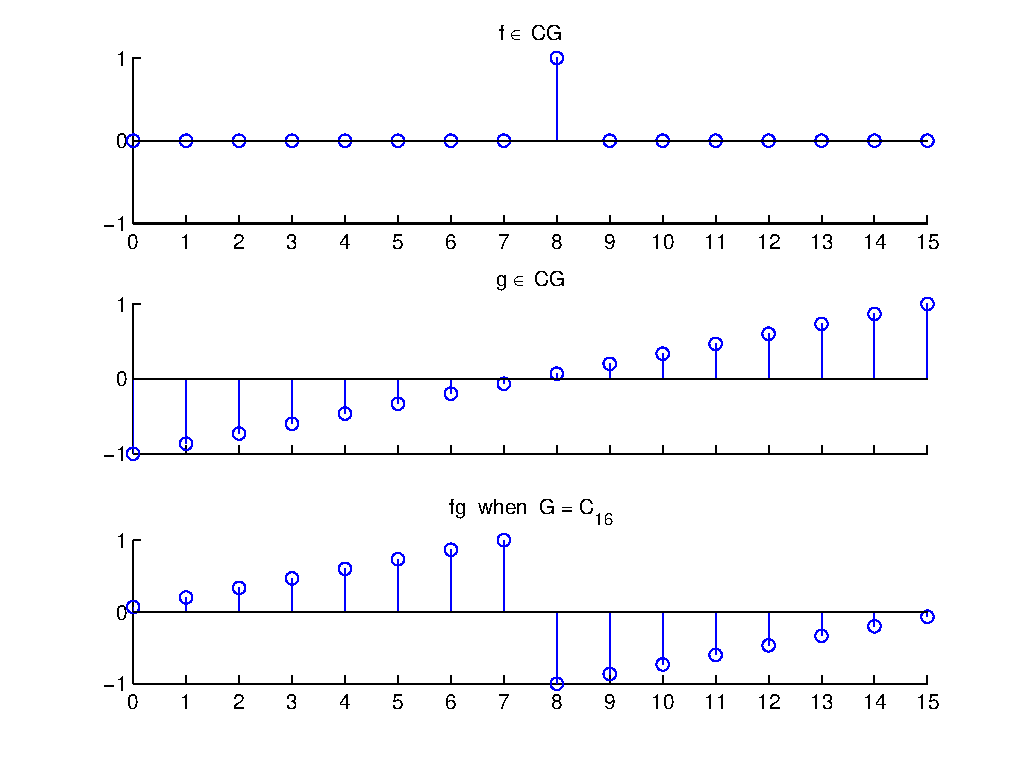
\includegraphics[width=\columnwidth, height=75mm]{C16conv_1}}}
\caption{Convolution of two signals indexed by the abelian
  group $C_{16}$.}
\label{fig:C16conv}
\end{figure}

Fig.~\ref{fig:k7conv} shows the convolution $C(f)g = fg$,
where $f$ is an impulse at the 9th sample, with group index $k_7$, and
$g$ is a linearly increasing sequence of 16 numbers ranging
from -1 to 1; $g$ can be represented as a vector,
or as an element of the group algebra $\C(C_8 \sdp \{1, k_7\})$,
\[
g = \sum_{m=0}^7 \sum_{j=0}^1 g(x^mk_7^j) x^mk_7^j
\]
with coefficients $g(x^mk_7^j)$ taking the values given
in~(\ref{eq:gvec}); \ie 
\[
g(1)=-1, \, g(x)=-0.8\bar{6}, %\, g(x^2)=-0.7\bar{3},
\ldots, g(x^7)=-0.0\bar{6},
\]
\[
g(k_7)=0.0\bar{6}, \, g(x k_7)=0.2, \ldots, g(x^7 k_7) = 1.
\]

\begin{figure}
\centerline{\framebox{
	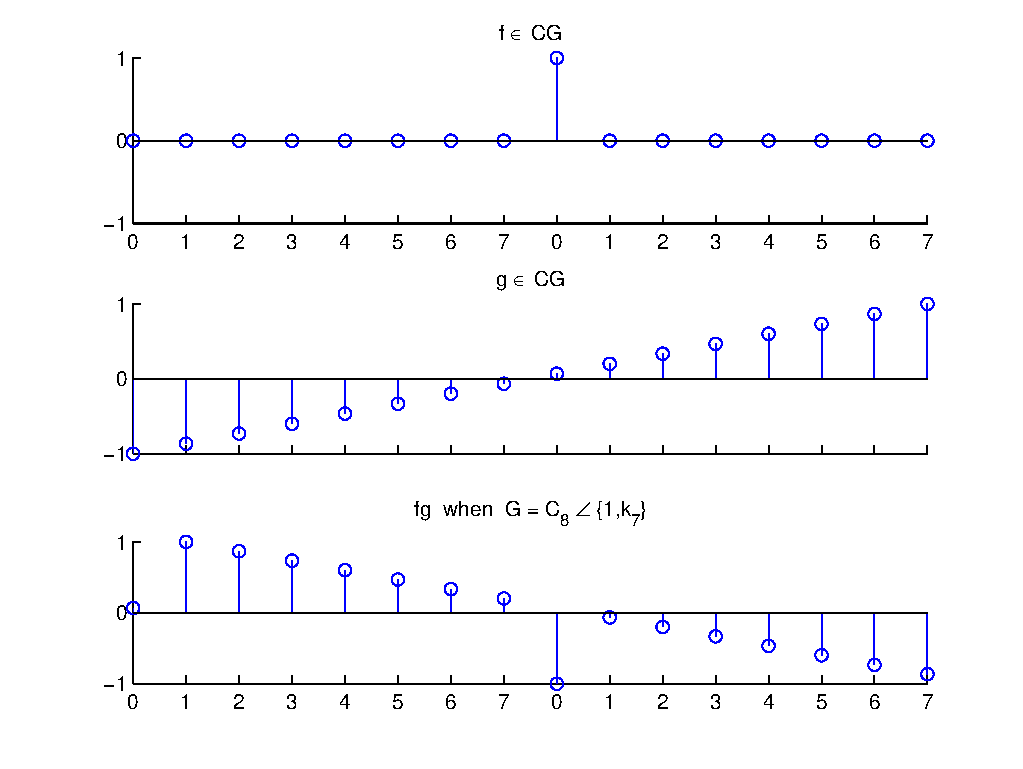
\includegraphics[width=\columnwidth, height=75mm]{k7conv_1}}}
\caption{The element $k_{N-1} \in G$ (top), where $N=8$ and $G = C_{8}\sdp \{1,k_7\}$ -- as an element of the group
  algebra, $f =  k_7 \in \CG$ is the ``impulse 
    function'' with one nonzero coefficient $f(k_7) =1$; 
    A linear signal $g\in \CG$ (middle); the product $fg = k_7g$ (bottom) is,
    in general, the convolution of $g$ by $f$, and is implemented
    by appealing to the convolution theorem and using a 
    generalized FFT algorithm.}
%\caption{Convolution of two signals indexed by the nonabelian
%  group $C_{8}\sdp \{1,k_7\}$.}
\label{fig:k7conv}
\end{figure}

\begin{figure}
\centerline{\framebox{
	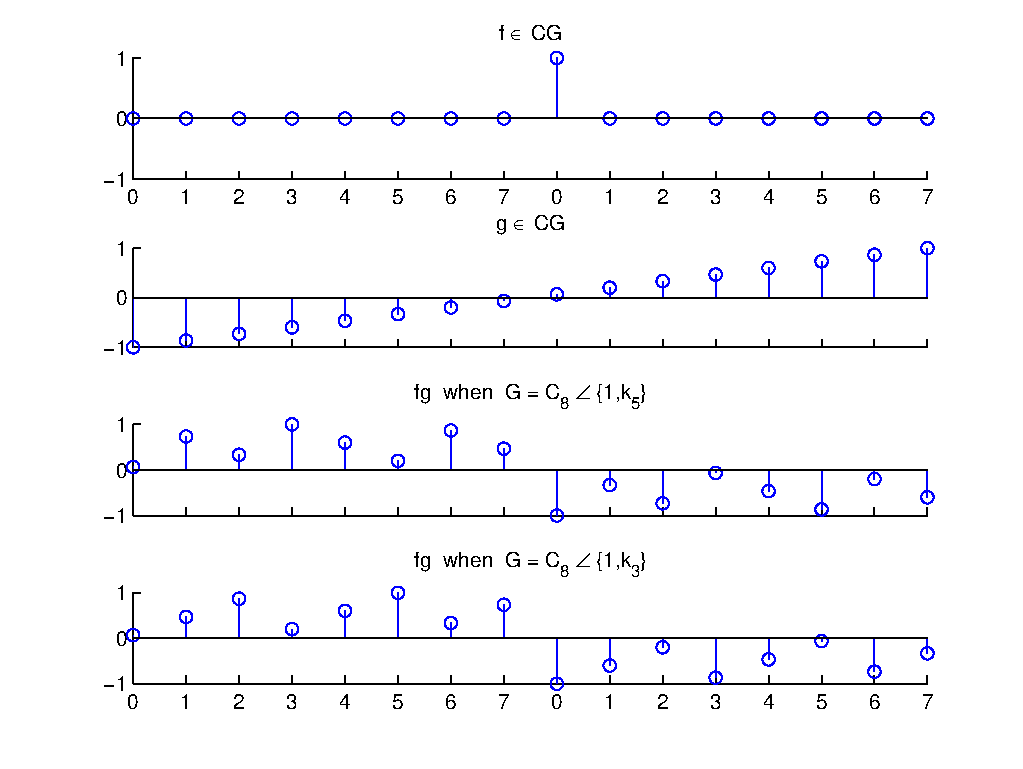
\includegraphics[width=\columnwidth, height=75mm]{k5_k3_conv_1}}}
\caption{Convolution of two signals indexed by the nonabelian
  groups $C_{8}\sdp \{1,k_5\}$ (third graph) and 
  $C_{8}\sdp \{1,k_5\}$ (fourth graph).}
\label{fig:k5_k3_conv}
\end{figure}


%=======================================================================
\subsection{Examples: 2-D Semidirect Product Indexing Sets}%\protect\footnotemark}
%=======================================================================
%\footnotetext{An and Tolimieri (2003), page 125.}
\begin{example}
Recall that $\lt{GL}(2,\Z/N)$ denotes the set of all $2\times 2$ invertible
matrices with coefficients in $\Z/N$.  
For $c\in \lt{GL}(2,\Z/N)$ such that $c^M$ is the identity,
%in $\lt{GL}(2,\Z/N)$ -- 
consider the \emph{action group} $K_c$ defined by
\[
C_M(k_c) = \{k_c^m : 0 \leq m < M\}, \quad
c = \begin{pmatrix} c_0 & c_1 \\ c_2 & c_3 \end{pmatrix}
%\in \lt{GL}(2,\Z/N).
\]
The semidirect product of $H$ and $K_c$ has elements
\[
H\varangle K_c = \{x^j y^k k_c^m : 0 \leq j,k < L, 0 \leq m< M\}
\]
and binary composition satisfying the following relations:
\[
x^L = y^L = k_c^M = 1,
\]
\[
x^{-1} = x^{L-1}, \quad y^{-1}= y^{L-1}, \quad k_c^{-1} = k_c^{M-1},
\]
\[
k_c x^j y^k = x^{c_0 j + c_1 k} y^{c_2 j + c_3 k} k_c.
\]
where the summands in the exponents are modulo $|H|=L$.
\end{example}

\subsection{Example: 2-D Rotations.} \textcolor{red}{\bf DEBUG this subsection.}\\

Let $A = C_N(x) \times C_N(y)$ with binary composition satisfying
\[
(x^my^j)(x^ny^k) = x^{m+n \bmod N}y^{j+k \bmod N},
\]
\[
%x^N = (x^N,1) = (1,1) = 1, \quad y^N = (1,y^N) = (1,1) = 1
x^N = y^N = 1, \quad x^{-1} = x^{N-1}, \quad y^{-1}= y^{N-1}.
\]
%\[x^{-1} = x^{N-1}, \quad y^{-1}= y^{N-1}.\]
Consider the action group $K_c$, $c\in \lt{GL}(2,\Z/N)$,
%\[c = \begin{pmatrix} c_0 & c_1 \\ c_2 & c_3 \end{pmatrix}.\]
with $c^M=1$.
%\ie $c^M = \begin{pmatrix} 1 & 0 \\ 0 & 1 \end{pmatrix}$.
%\ie \[\begin{pmatrix} c_0 & c_1 \\ c_2 & c_3 \end{pmatrix}^M
%= \begin{pmatrix} 1 & 0 \\ 0 & 1 \end{pmatrix}\]
The group generated by $k_c$ is the cyclic group of order
$M$ with elements $C_M(k_c) = \{k_c^m : 0 \leq m < M\}$.
Now suppose
\[
c(\theta) = \begin{pmatrix} \cos \theta \, &  -\sin \theta \\ 
                    \sin \theta \, & \, \cos \theta \end{pmatrix}.
\]
\begin{example}[Rotation by $\pi/2$]
The action group $K_{c(\pi/2)}$ has
\[
c(\pi/2) = \begin{pmatrix} 0\, & -1\\ 
                            1\, & \, 0 \end{pmatrix}.
\]
Since $c^4(\pi/2)$ is the identity, the group
has order $M=4$.
\end{example}

The semidirect product $A\varangle K_{c(\theta)}$ has elements
$\{x^j y^k k_{c(\theta)}^m : 0 \leq j,k < N,\, 0 \leq m < M\}$,
and binary composition satisfying
\[
x^N = y^N = k_{c(\theta)}^M = 1,
\]
\[
x^{-1} = x^{N-1}, \quad y^{-1}= y^{N-1}, \quad k_{c(\theta)}^{-1} = k_{c(\theta)}^{M-1},
\]
and
\[
k_{c(\theta)} x^j y^k = x^{j \cos \theta - k \sin \theta} y^{j \sin
  \theta + k \cos \theta} k_{c(\theta)},
\]
Additive operations in the exponents are modulo $|A|=N$.

We now demonstrate the effect of successive left
multiplications by the $k_c$ described above.  
%on an array representaion of an image $f$.  
Suppose an image $f$ has the following array representation:
{\footnotesize
\begin{equation*}
\left(
\begin{array}{cccc|cccc|cccc|cccc}
%\begin{array}{rrrr|rrrr|rrrr|rrrr}
0&0& 0  & 0 & 0 & 0 & 0 & 0 & 0 & 0 & 0 & 0 & 0 & 0 & 0 & 0 \\ 
0&10& 12 & 2 & 0 & 1 & 1 & 1 & 0 & 2 & 2 & 2 & 0 & 3 & 3 & 3 \\ 
0&9& 0  & 3 & 0 & 1 & 1 & 1 & 0 & 2 & 2 & 2 & 0 & 3 & 3 & 3 \\ 
0&8& 6  & 4 & 0 & 1 & 1 & 1 & 0 & 2 & 2 & 2 & 0 & 3 & 3 & 3 
\end{array}\right)
\end{equation*}
}
Notice that, in the left-most $4\times 4$ block of this
array, there is a $3\times 3$ subarray with entries
approximating the locations on the face of an analog clock.  
%These are the numbers on which we focus while left
%multiplication by $k_c$ transforms the entire array, 
%since they 
Such a configuration facilitate our observation of the local
behavior of the non-abelian group translation -- that is,
the action of $k_c$ on the elements within the given
$4\times 4$ block.  The subarrays of the 
three other $4\times 4$ blocks are designed to reveal the
global effect of the non-abelian translation.  That is, they
demonstrate how the blocks shift around (though the
elements within each of these blocks undergo the same
transformation as those of the first block.)
%observe this intrablock behavior since the numbers are all the same.)

The following are the array representations of $k_c f, \, k_c^2 f$, and $k_c^3 f$, resp. 
{\footnotesize
\begin{equation*}
\left(
\begin{array}{cccc|cccc|cccc|cccc}
0 & 0 & 0 & 0 & 0 & 0  & 0 & 0 & 0 & 0 & 0 & 0 & 0 & 0 & 0 & 0 \\ 
0 & 3 & 3 & 3 & 0 & 2  & 3 & 4 & 0 & 1 & 1 & 1 & 0 & 2 & 2 & 2 \\ 
0 & 3 & 3 & 3 & 0 & 12 & 0 & 6 & 0 & 1 & 1 & 1 & 0 & 2 & 2 & 2 \\ 
0 & 3 & 3 & 3 & 0 & 10 & 9 & 8 & 0 & 1 & 1 & 1 & 0 & 2 & 2 & 2 
\end{array}\right)
\end{equation*}
\begin{equation*}
\left(
\begin{array}{cccc|cccc|cccc|cccc}
0 & 0 & 0 & 0 & 0 & 0 & 0 & 0 & 0 & 0 & 0  & 0  & 0 & 0 & 0 & 0 \\ 
0 & 2 & 2 & 2 & 0 & 3 & 3 & 3 & 0 & 4 & 6  & 8  & 0 & 1 & 1 & 1 \\ 
0 & 2 & 2 & 2 & 0 & 3 & 3 & 3 & 0 & 3 & 0  & 9  & 0 & 1 & 1 & 1 \\ 
0 & 2 & 2 & 2 & 0 & 3 & 3 & 3 & 0 & 2 & 12 & 10 & 0 & 1 & 1 & 1 
\end{array}\right)
\end{equation*}
\begin{equation*}
\left(
\begin{array}{cccc|cccc|cccc|cccc}
0 & 0 & 0 & 0 & 0 & 0 & 0 & 0 & 0 & 0 & 0 & 0 & 0 & 0 & 0 & 0 \\ 
0 & 1 & 1 & 1 & 0 & 2 & 2 & 2 & 0 & 3 & 3 & 3 & 0 & 8 & 9 & 10 \\ 
0 & 1 & 1 & 1 & 0 & 2 & 2 & 2 & 0 & 3 & 3 & 3 & 0 & 6 & 0 & 12 \\ 
0 & 1 & 1 & 1 & 0 & 2 & 2 & 2 & 0 & 3 & 3 & 3 & 0 & 4 & 3 & 2 
\end{array}\right)
\end{equation*}
}

\subsection{Digital lines}
\textcolor{red}{\bf DEBUG this subsection.}\\
This section defines digital lines and the Matlab
routines used to process them. Such examples are useful
for demonstrating the nature of the generalized
translations and convolutions that are possible when 
the groups used to index the data are nonabelian.

\begin{figure}[t]               
%  \ifthenelse{\boolean{nofigures}}{}{
    \centering  
    \includegraphics[width=\columnwidth]{fline1}
%  }
  \caption{{\it Figures 10.4.1--10.4.3 of An (2003),
      re-produced with {\tt fline.m} program.}}  
  \label{fig:10.4.1}
\end{figure}

\begin{figure}[t]
%  \ifthenelse{\boolean{nofigures}}{}{
    \centering  
    \includegraphics[width=\columnwidth]{fline2}
%  }
    \caption{{\it Figures 10.4.4--10.4.6 of An (2003)
        re-produced with {\tt fline.m} program.}}  
  %% (see figures 10.4.4--10.4.6 in An & Tolimieri, pages 216--218)
  \label{fig:10.4.4}
\end{figure}

\begin{figure}
    \centering  
    \includegraphics[width=\columnwidth]{1234trans}
  \caption{Translates of an image in 
  $(C_N(x)\times C_N(y)) \sdp (K_a \times K_b)$.} 
  \label{fig:1234trans}
\end{figure}


%\begin{figure}[t]               
%%  \ifthenelse{\boolean{nofigures}}{}{
%    \centering  
%    \includegraphics[width=100mm]{1234trans}
%%  }
%  \caption{{\it Translates of an image in $G_1$.}}
%  \label{fig:1234trans}
%\end{figure}






%\verb!\input{Appendix/hafg}!
%\input{Appendix/hafg}
%\verb!\input{hafg/old/notation}!
%\input{hafg/old/notation}
%\verb!\input{hafg/old/nonabelianDSP}!
%\input{hafg/old/nonabelianDSP}
%\verb!\input{hafg/old/sdp}!
%\input{hafg/old/sdp}
%\verb!\input{hafg/old/examples}!
%\input{hafg/old/examples}
%\verb!\input{hafg/old/summary}!

% Reminder: the "draftcls" or "draftclsnofoot", not "draft", class option
% should be used if it is desired that the figures are to be displayed while
% in draft mode.

% An example of a floating figure using the graphicx package.
% Note that \label must occur AFTER (or within) \caption.
% For figures, \caption should occur after the \includegraphics.
%
%\begin{figure}
%\centering
%\includegraphics[width=2.5in]{myfigure}
% where an .eps filename suffix will be assumed under latex, 
% and a .pdf suffix will be assumed for pdflatex
%\caption{Simulation Results}
%\label{fig_sim}
%\end{figure}


% An example of a double column floating figure using two subfigures.
% (The subfigure.sty package must be loaded for this to work.)
% The subfigure \label commands are set within each subfigure command, the
% \label for the overall fgure must come after \caption.
% \hfil must be used as a separator to get equal spacing
%
%\begin{figure*}
%\centerline{\subfigure[Case I]{\includegraphics[width=2.5in]{subfigcase1}
% where an .eps filename suffix will be assumed under latex, 
% and a .pdf suffix will be assumed for pdflatex
%\label{fig_first_case}}
%\hfil
%\subfigure[Case II]{\includegraphics[width=2.5in]{subfigcase2}
% where an .eps filename suffix will be assumed under latex, 
% and a .pdf suffix will be assumed for pdflatex
%\label{fig_second_case}}}
%\caption{Simulation results}
%\label{fig_sim}
%\end{figure*}



% An example of a floating table. Note that, for IEEE style tables, the 
% \caption command should come BEFORE the table. Table text will default to
% \footnotesize as IEEE normally uses this smaller font for tables.
% The \label must come after \caption as always.
%
%\begin{table}
%% increase table row spacing, adjust to taste
%\renewcommand{\arraystretch}{1.3}
%\caption{An Example of a Table}
%\label{table_example}
%\centering
%% Some packages, such as MDW tools, offer better commands for making tables
%% than the plain LaTeX2e tabular which is used here.
%\begin{tabular}{|c||c|}
%\hline
%One & Two\\
%\hline
%Three & Four\\
%\hline
%\end{tabular}
%\end{table}

%
% \input{hafg/old/summary}
